\begin{frame}
\frametitle{Note}
\begin{itemize}
\item This is a document which combines all materials from the Scheduling course
\item Files as also available individually in separate directories
\end{itemize}
\end{frame}

\begin{frame}
\frametitle{Insight is one of the largest data research and innovation centres in Europe...}
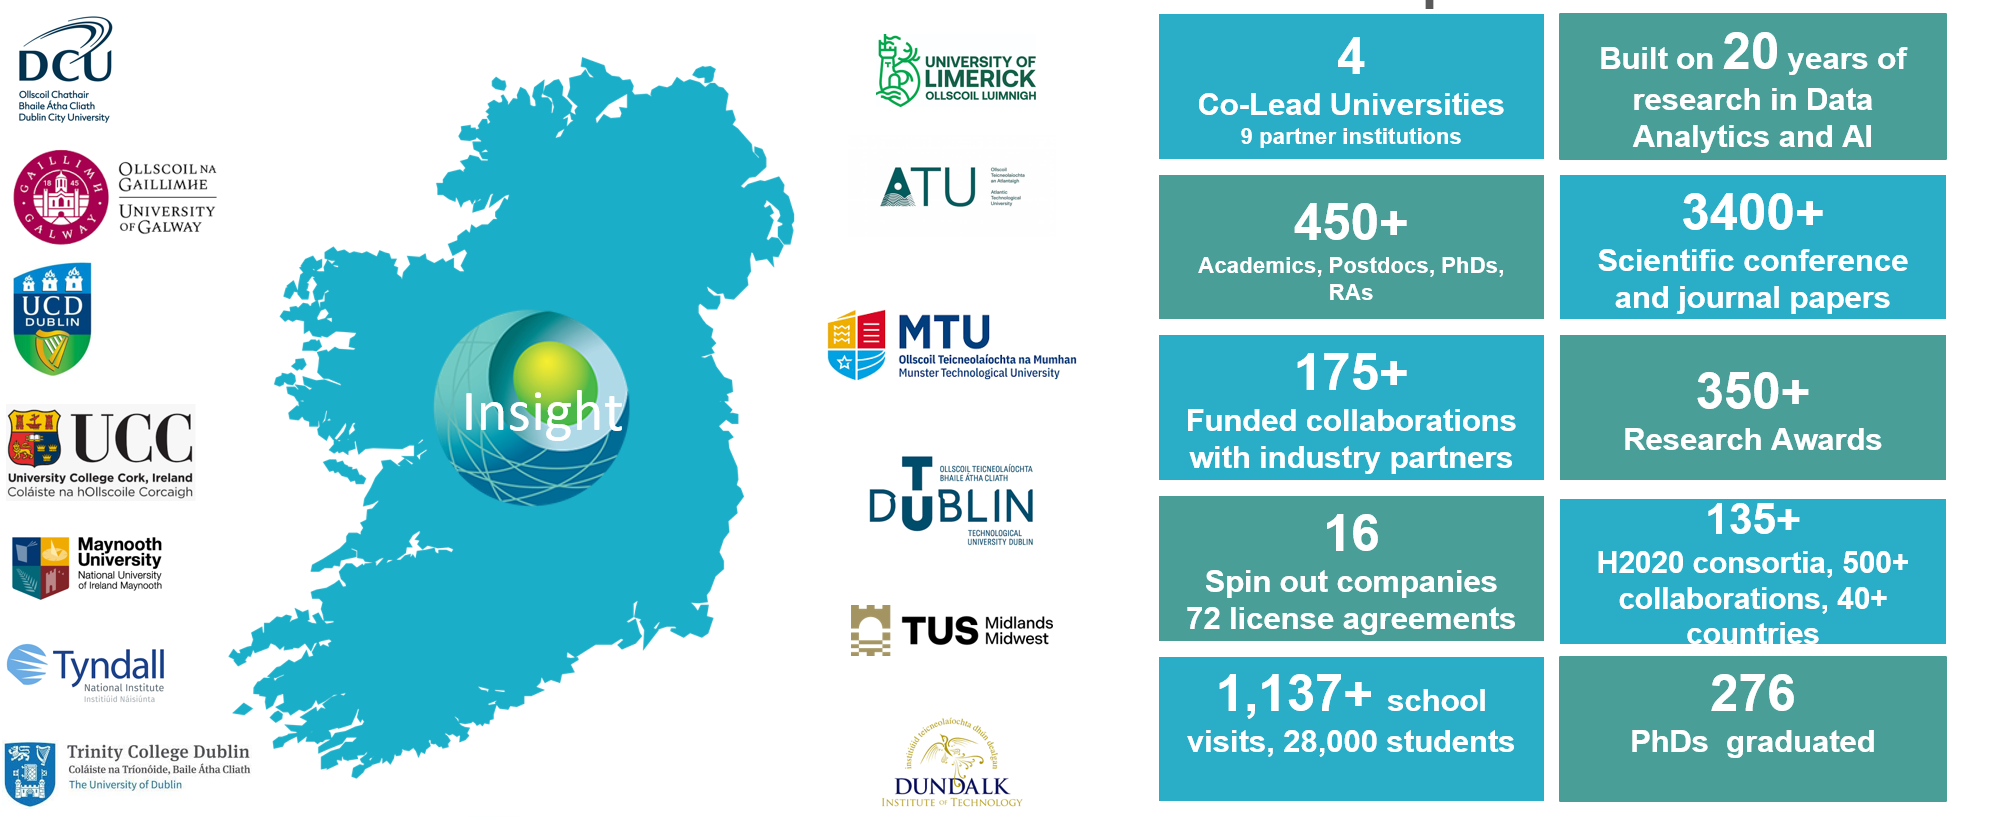
\includegraphics[width=\textwidth]{../book/images/onepage}
\end{frame}

\begin{frame}[fragile]
\frametitle{Rinn Artificial Intelligence: Research \& Innovation in Data Science and AI}
\begin{columns}
\begin{column}{0.65\textwidth}
\begin{quotation}
Rinn Artificial Intelligence is designed to serve as a national hub for research and innovation in data science and AI. The programme has two overarching goals: (i) to advance foundational cutting-edge research in Data Science and AI, and (ii) to pursue open, international, and inter- and transdisciplinary research aimed at studying, designing, and implementing strategies to address societal challenges.
\end{quotation}
\end{column}
\begin{column}{0.35\textwidth}

\includegraphics[width=.85\textwidth]{../book/images/rinnailogo}
\end{column}
\end{columns}
\end{frame}

\begin{frame}
\frametitle{Background}
\begin{columns}
\begin{column}{0.70\textwidth}
\begin{itemize}
\item Mathematics @ TH Darmstadt
\item 1986-1990 ECRC GmbH, Munich
\item 1990-2000, Technical Director, Cosytec SA, Orsay
\item 2000-2005, Imperial College London, Parc Technologies Ltd
\item 2013-2014, President, Association for Constraint Programming
\item Best Application Paper Awards, CP 2009, CP 2013
\item Program Chair, CP 2020, CPAIOR 2014
\item Distinguished Service Award, ACP
\item Editor in Chief, Constraints, 2026
\end{itemize}
\end{column}
\begin{column}{0.30\textwidth}
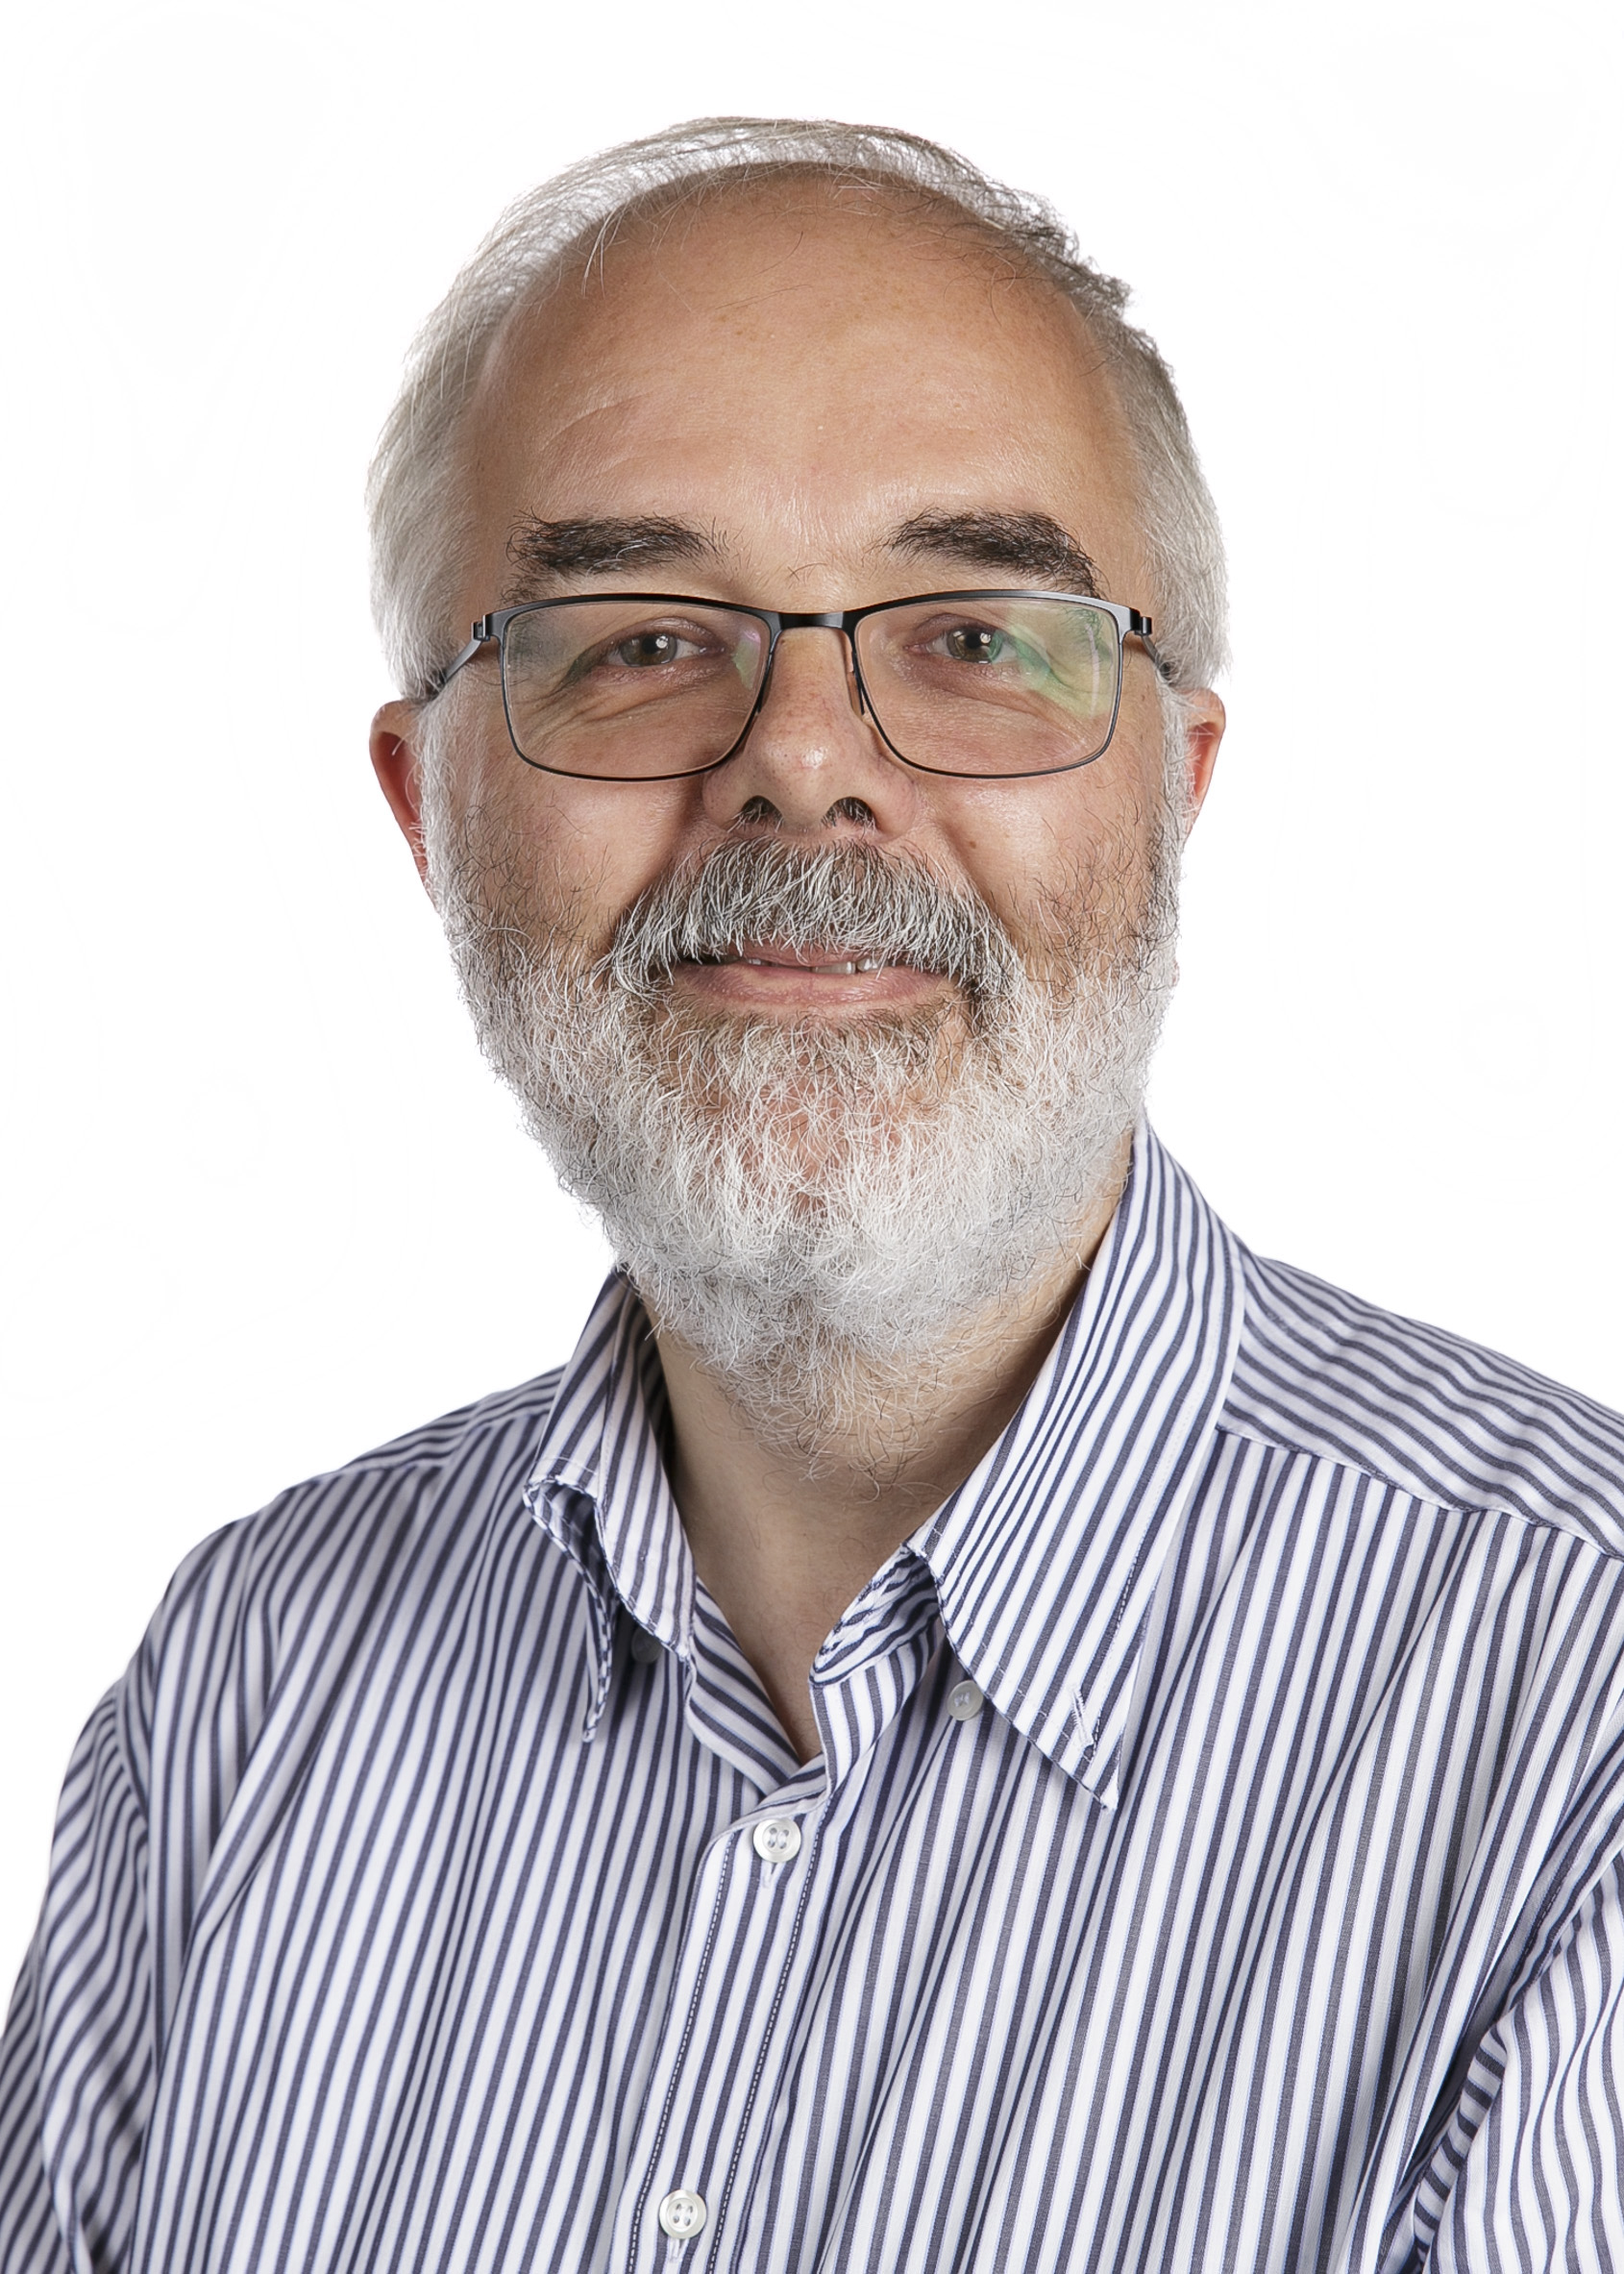
\includegraphics[width=.85\textwidth]{../book/images/helmut}
\end{column}
\end{columns}
\end{frame}

\begin{frame}
\frametitle{Course Structure}
\begin{tabular}{lp{9cm}}\toprule
Time & Topic \\\midrule
09:00-09:30 & Registration \& Welcome \\
09:30-10:30 & Introduction \& Motivation\\
10:30-11:00 & Coffee \\
11:00-12:30 & Scheduling Concepts\\
12:30-13:30 & Lunch\\
13:30-15:00 & Case Studies\\
15:00-15:30 & Coffee \\
15:30-16:30 & Hands-on Experience\\
\bottomrule
\end{tabular}
\end{frame}
